\newpage
\section{Diagramme de Cas d'Utilisation}\label{sec:diagramme_casutilisation}
\begin{definition}[Diagramme de Cas d'Utilisation]
Un diagramme de cas d'utilisation (Use Case Diagram) est une type de diagramme UML qui représente un ensemble de cas d'utilisation, ses acteurs et leurs relations dans le but de réaliser une fonctionnalité spécifique.
Un diagramme de cas d'utilisation est un type de diagramme UML qui représente les interactions entre les acteurs et le système en vue de réaliser une tâche spécifique. 
\end{definition}
\begin{definition}[Cas d'utilisation]
Un cas d'utilisation est une description des interactions entre un système et ses utilisateurs dans le but de réaliser une tâche spécifique.
\end{definition}
\begin{definition}[Cas d'utilisation d'extension]
Un cas d'utilisation d'extension est une spécification qui décrit un cas d'utilisation qui peut étendre ou modifier le comportement d'un cas d'utilisation principal en cas de conditions exceptionnelles ou conditionnelles.
\end{definition}


\begin{table}[H]
	\caption{\'El\'ements constitutifs d'un diagramme de cas d'utilisation}
	\label{tbl:diagram_usecase_elements}
	\begin{adjustbox}{max width=\textwidth}
		\begin{tabular}{l|p{40em}}
			\toprule
			\textbf{\'El\'ements} & \textbf{Repr\'esentation}\\
			\midrule
			Acteur & Représenté par une personne ou une entité extérieure au système. \\
			Cas d'utilisation & Représenté par une ellipse et décrivant une fonctionnalité du système. \\
			Liens & Représenté par une flèche reliant l'acteur au cas d'utilisation. \\
			Condition d'inclusion & Représentée par une flèche avec des traits en pointillé reliant un cas d'utilisation principal à un cas d'utilisation d'inclusion et indiquant une fonctionnalité inclue. \\
			Condition d'extension & Représentée par une flèche avec des traits en pointillé reliant un cas d'utilisation d'extension à un cas d'utilisation  principal et indiquant une fonctionnalité supplémentaire qui peut être réalisée dans certains cas spéciaux.\\
			Généralisation & Représentée par une flèche reliant la spécialisation à la généralisation. \\
			\bottomrule
	\end{tabular}
	\end{adjustbox}
\end{table}

\begin{figure}[H]
	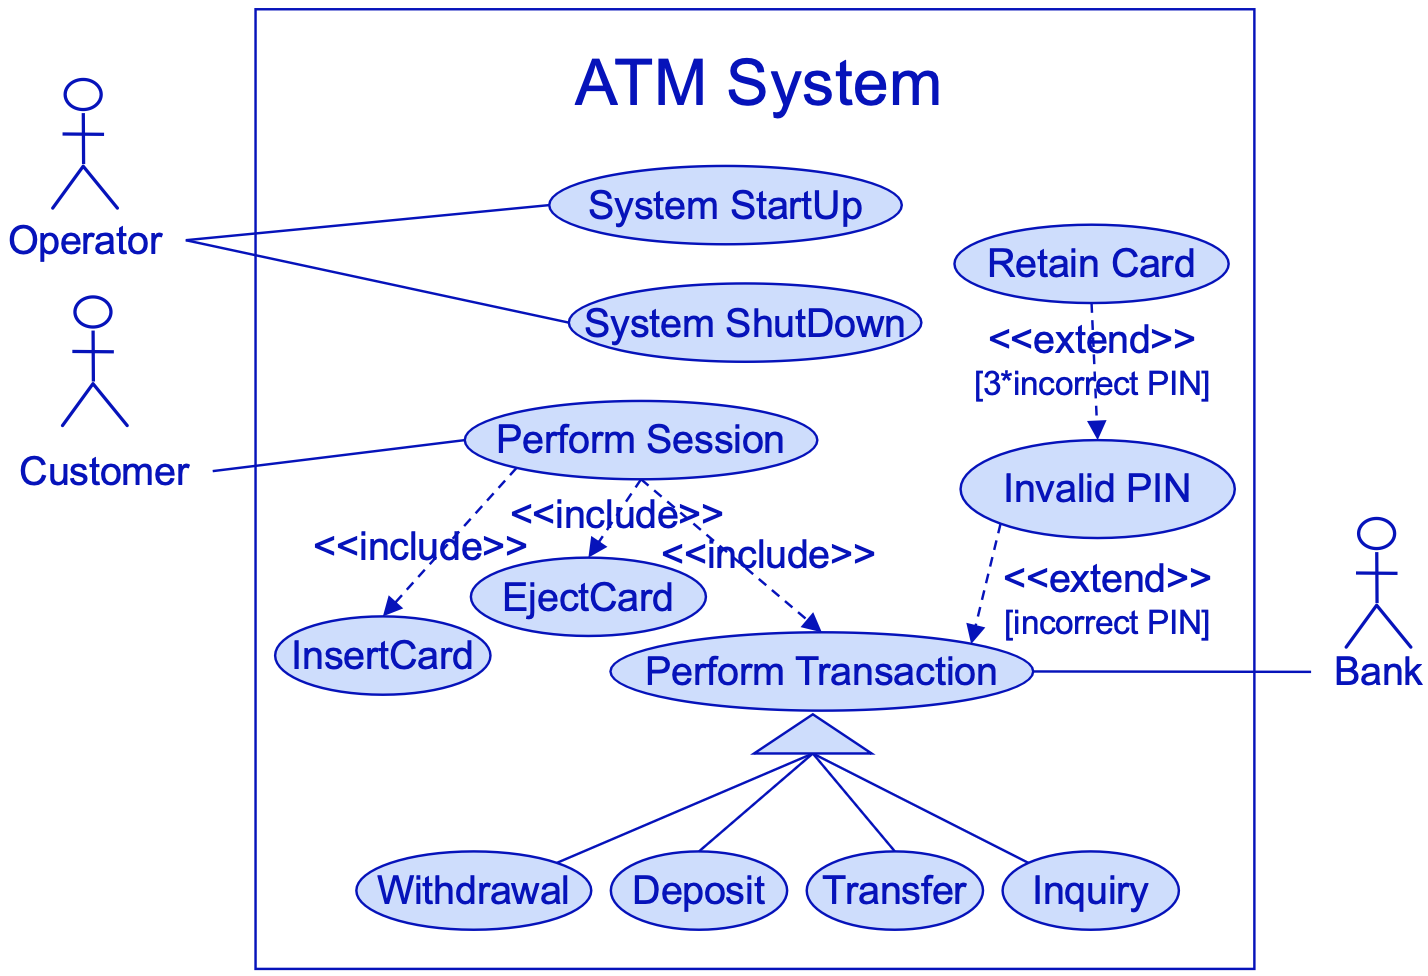
\includegraphics[width=\textwidth]{./Images/Diagrammes/diagram_usecase_ex_atm.png}
	\caption{Exemple de diagramme de cas d'utilisation : ATM.}
	\label{fig:diagram_usecase_ex_atm}
\end{figure}

\newpage
